\documentclass[11pt, fleqn]{article}

\documentclass[11pt, fleqn]{article}

\usepackage[usenames,dvipsnames,svgnames,table]{xcolor}
\usepackage{amsmath}
\usepackage{amsfonts}
\usepackage[margin=1in]{geometry} % To set the margin widths
\usepackage{graphicx}
\usepackage{listings}
\usepackage{multirow}
\usepackage{tabularx}
\usepackage{varioref}
\usepackage[noabbrev,capitalize]{cleveref}
\usepackage[group-separator={,}]{siunitx}
\usepackage{subcaption}
\usepackage{titlesec}
\usepackage{lscape}
\usepackage{bm}
\usepackage[titletoc,toc,title]{appendix}

\lstset{
  frame=single,
  basicstyle=\ttfamily,% print whole listing small
  language=R,
  aboveskip=3mm,
  belowskip=3mm,
  showstringspaces=false,
  columns=flexible,
  numbers=none,
  commentstyle=\color{ForestGreen},
  stringstyle=\color{Maroon},
  breaklines=true,
  breakatwhitespace=true,
  tabsize=2,
  literate={<-}{{$\gets$}}1 {~}{{$\sim$}}1
}

\sisetup{output-exponent-marker=\textsc{e}}

\setlength{\parskip}{12pt} % Sets a blank line in between paragraphs
\setlength\parindent{0pt} % Sets the indent for each paragraph to zero

% \crefname{figure}{Figure}{Figures}
% \crefname{section}{Section}{Sections}
% \crefname{table}{Table}{Tables}
% \crefname{lstlisting}{Listing}{Listings}

\setlength{\parskip}{12pt} % Sets a blank line in between paragraphs
\setlength\parindent{0pt} % Sets the indent for each paragraph to zero

\begin{document}

\title{Machine Learning (41204-01)\\HW \#2}
\author{Will Clark $\vert$ Matthew DeLio \\
\texttt{will.clark@chicagobooth.edu} $\vert$ \texttt{mdelio@chicagobooth.edu} \\
University of Chicago Booth School of Business}
\date{\today}
\maketitle

\section{kNN with 1 Attribute}

In the previous assignment, we chose a k-nearest neighbors algorithm with a value of $k=40$. In this exercise, we will use 5-fold cross validation to chose $k$ in a more systematic manner. In \cref{fig:1p_k}, we show the average root mean square error (RMSE) for each of five folds over values of $k \in (2,300)$. The thick red line shows the average RMSE for each run with the minimum value highlighted at $k=28$. 

Because the training and test samples are being chosen randomly and because the number of folds is small, there is some run-to-run variation in the minimum $k$ selected with this method. To account for this, we can repeat 5-fold cross validation. Each trail will yield an optimal value of $k$, and we can look at the mean of this sequence of optimal $k$ values to determine the most optimal $k$ value.

We can see the effect of the number of folds on the \textit{distribution} of optimal $k$ values in \cref{fig:nfolds_k_dist}. We run 100 trials of cross validation for 5, 10, and 20 folds and show the distribution of optimal $k$ values as box plots. We can see that for 5-fold cross validation, the spread of optimal $k$ values is fairly high (as is the presence of outliers), but that the spread falls as the number of folds rises. 

\begin{figure}[!htb]
  \centering
  \caption{Distribution of Optimal k by Number of CV Folds}
  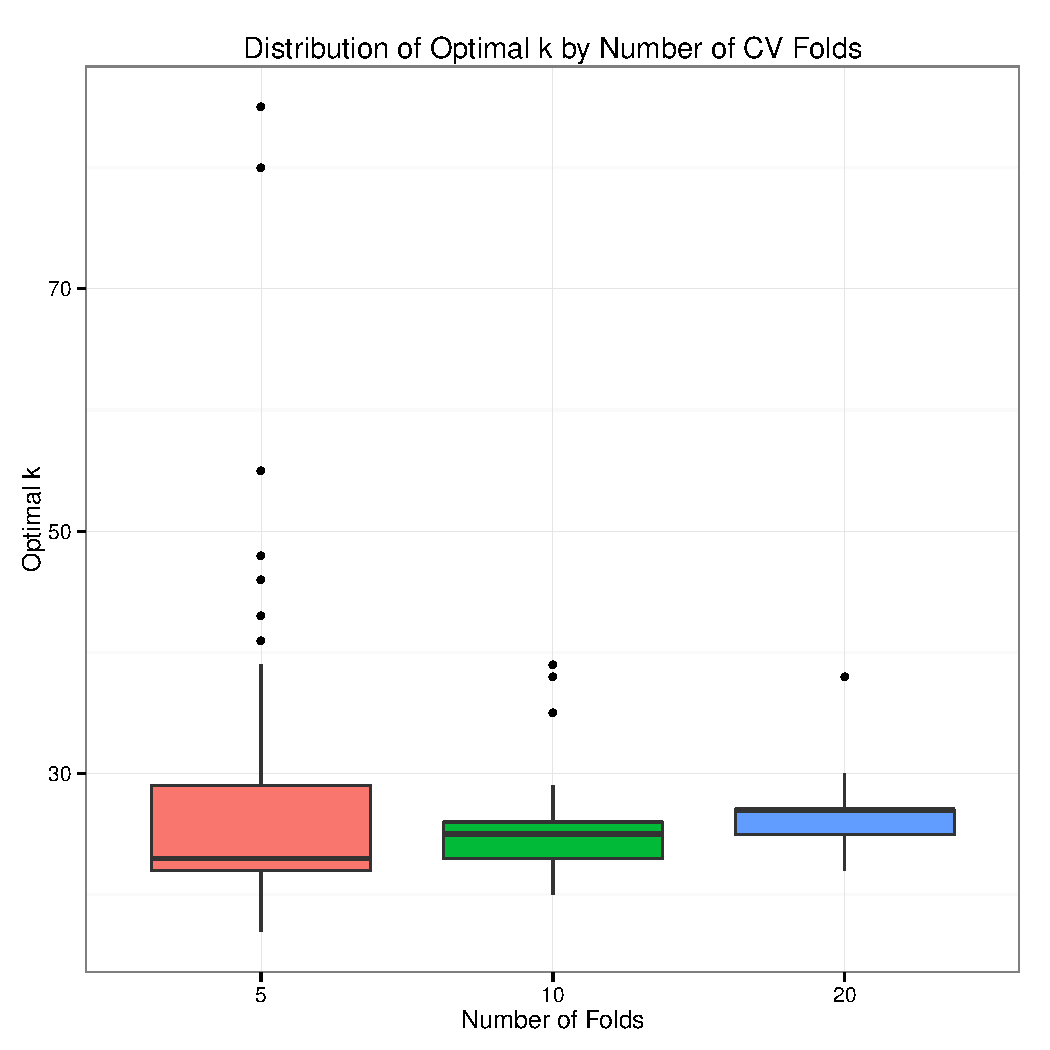
\includegraphics[scale=.5]{nfolds_k_dist.pdf}
  \label{fig:nfolds_k_dist}
\end{figure}

As it turns out, the mean optimal $k$ chosen over 100 trials of 5-fold cross validation is $k=27$, so our value of $k$ chosen over 1 run above is close to optimal. For the duration of the exercise we will use $k=28$ since the difference between the two model fits is negligible.

The difference between our ``eyeballed'' value of $k$ and the optimal value of $k$ discussed above is shown in \cref{fig:1p_fit}. The difference between the two is very small; the eyeballed value of $k=40$ provides a slightly smoother fit of the data, but by and large there is an insignificant difference between the fits.

\begin{figure}[!htb]
  \centering
  \caption{5-fold kNN CV for 1 Attribute}
  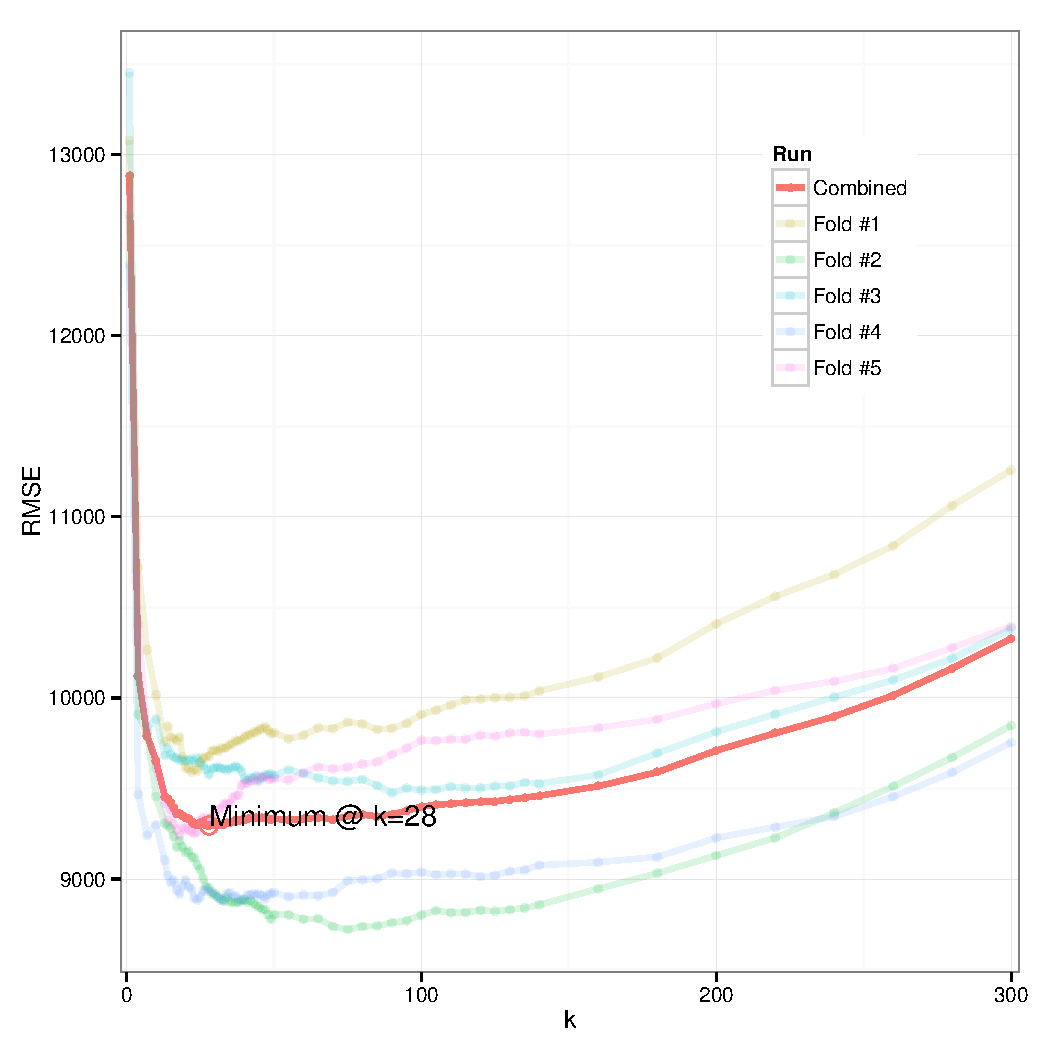
\includegraphics[scale=.5]{1p_cv_k.pdf}
  \label{fig:1p_k}
\end{figure}

\begin{figure}[!htb]
  \centering
  \caption{Comparison of Fit Between ``Eyeball'' and CV Chosen $k$'s}
  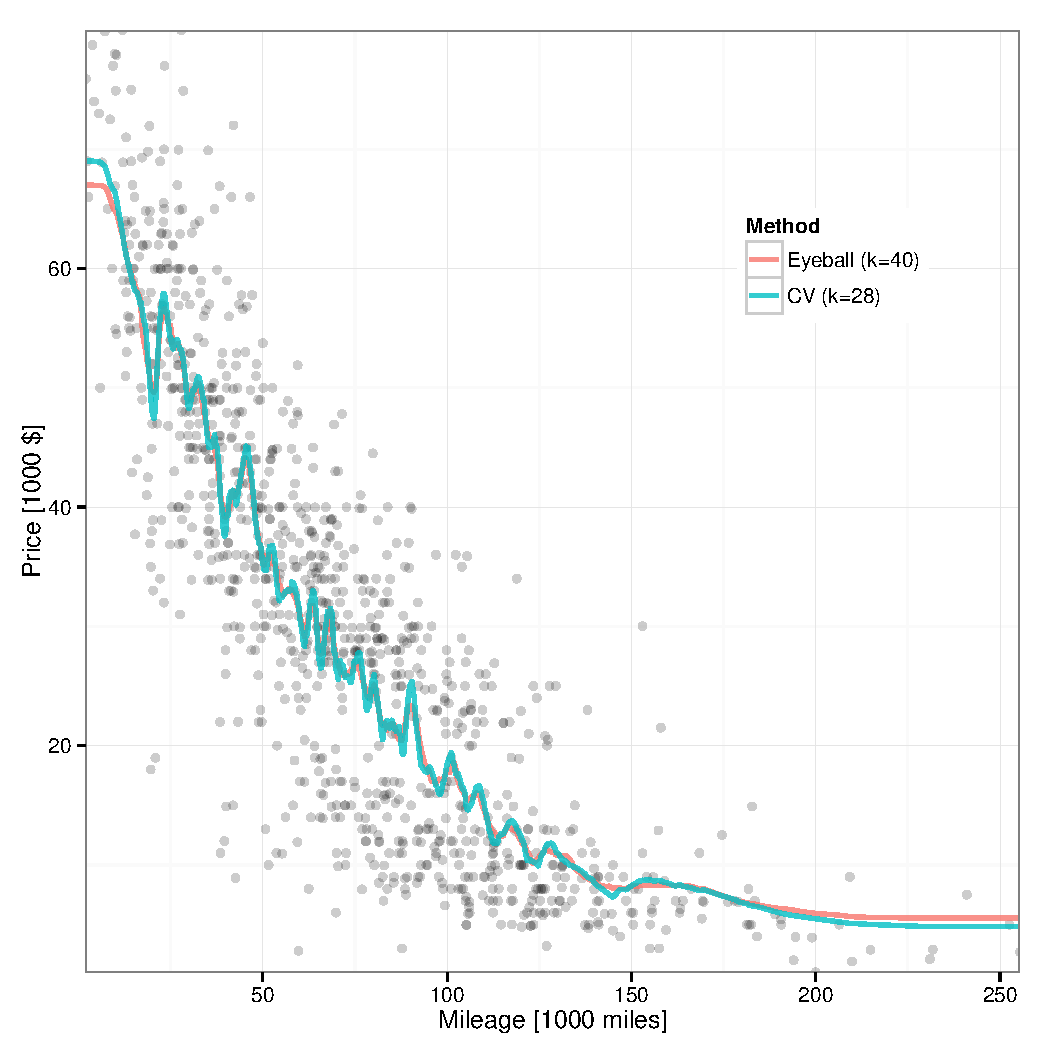
\includegraphics[scale=.5]{1p_fit_eye_ev.pdf}
  \label{fig:1p_fit}
\end{figure}

\subsection{Price Predictions}

Using the value of $k=28$ discussed above, our prediction for the price of a car with 100 thousand miles is \$16,676.18 (see \cref{tab:1p_predict}). We can see the predicted point in \cref{fig:1p_fit} outlined in black; it appears that the predicted value is well within the range of observed values for similar cars.

% latex table generated in R 3.1.2 by xtable 1.7-4 package
% Sun Oct  4 21:25:06 2015
\begin{table}[ht]
\centering
\begin{tabular}{rrr}
  \hline
 & Mileage & $\hat(price)$ \\ 
  \hline
1 & 100000 & 16676.18 \\ 
   \hline
\end{tabular}
\caption{Predicted Value with 1 Attribute} 
\label{tab:1p_predict}
\end{table}


\section{kNN with 2 Attributes}

In this section we explore the benefits of introducing a second attribute to our k-nearest neighbors algorithm. We will now use the car's mileage and its model year to predict is resale price.  To apply kNN to the data set we first examine the data-set and note that the two attributes used to predict price are on seemingly different scales.  In \cref{tab:data_scale} we see that the means are completely different and the standard deviations are also different. To avoid over-weighting one parameter with the other during model selection and prediction, these two attributes are independently scaled to ensure that $\mu_i=1$ and $\sigma_i^2=1$ using \cref{eq:scale}.  These scaled values are then used as inputs when training kNN.  When predicting prices, the inputs are scaled using the exact same parameters.

\begin{equation}\label{eq:scale}
x_{i,scaled} = \frac{x_i-\mu_i}{\sigma_i} 
\end{equation}

% latex table generated in R 3.1.2 by xtable 1.7-4 package
% Wed Oct  7 15:47:40 2015
\begin{table}[ht]
\centering
\begin{tabular}{lrr}
  \hline
column & mean & sd \\ 
  \hline
mileage & 73652.4 & 42887.4 \\ 
  year & 2006.9 & 4.2 \\ 
   \hline
\end{tabular}
\caption{Basic Dataset Statistics} 
\label{tab:data_scale}
\end{table}


With the resulting scaled inputs we run 5-fold cross-validated kNN, sweeping k from 1 to 300.\footnote{To save computation time, we focused our search by increasing the $k$ step-size in the range $k\in[14,50]$ reducing the step-size outside of this range.} \Cref{fig:2p_k} shows the mean and per-fold RMSE a single run of the cv kNN; here we find that RMSE is minimized with a choice of $k=23$.

\begin{figure}[!htb]
  \centering
  \caption{5-fold kNN CV for 2 Attributes}
  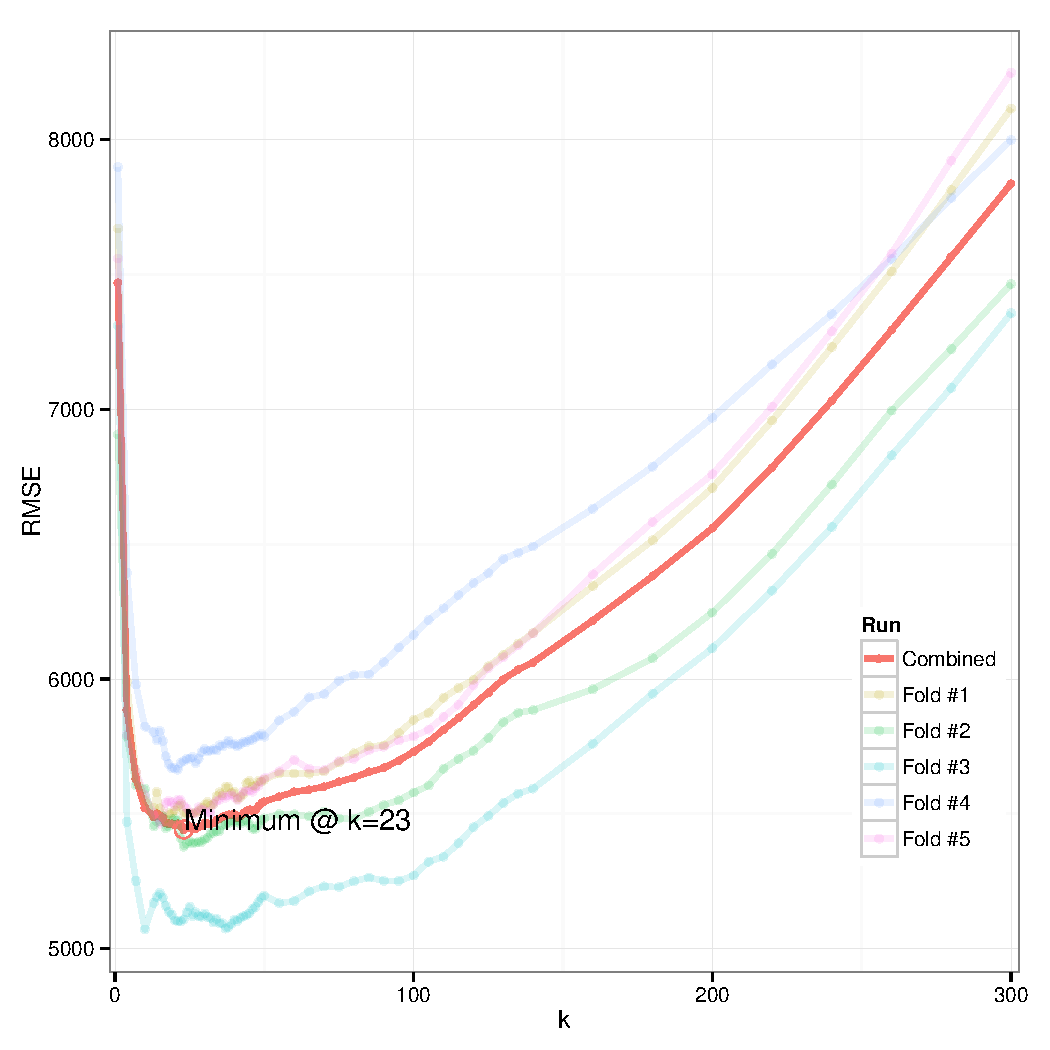
\includegraphics[scale=.5]{2p_cv_k.pdf}
  \label{fig:2p_k}
\end{figure}



\begin{figure}[!htb]
  \centering
  \caption{10-run 5-fold kNN CV average for 2 Attributes}
  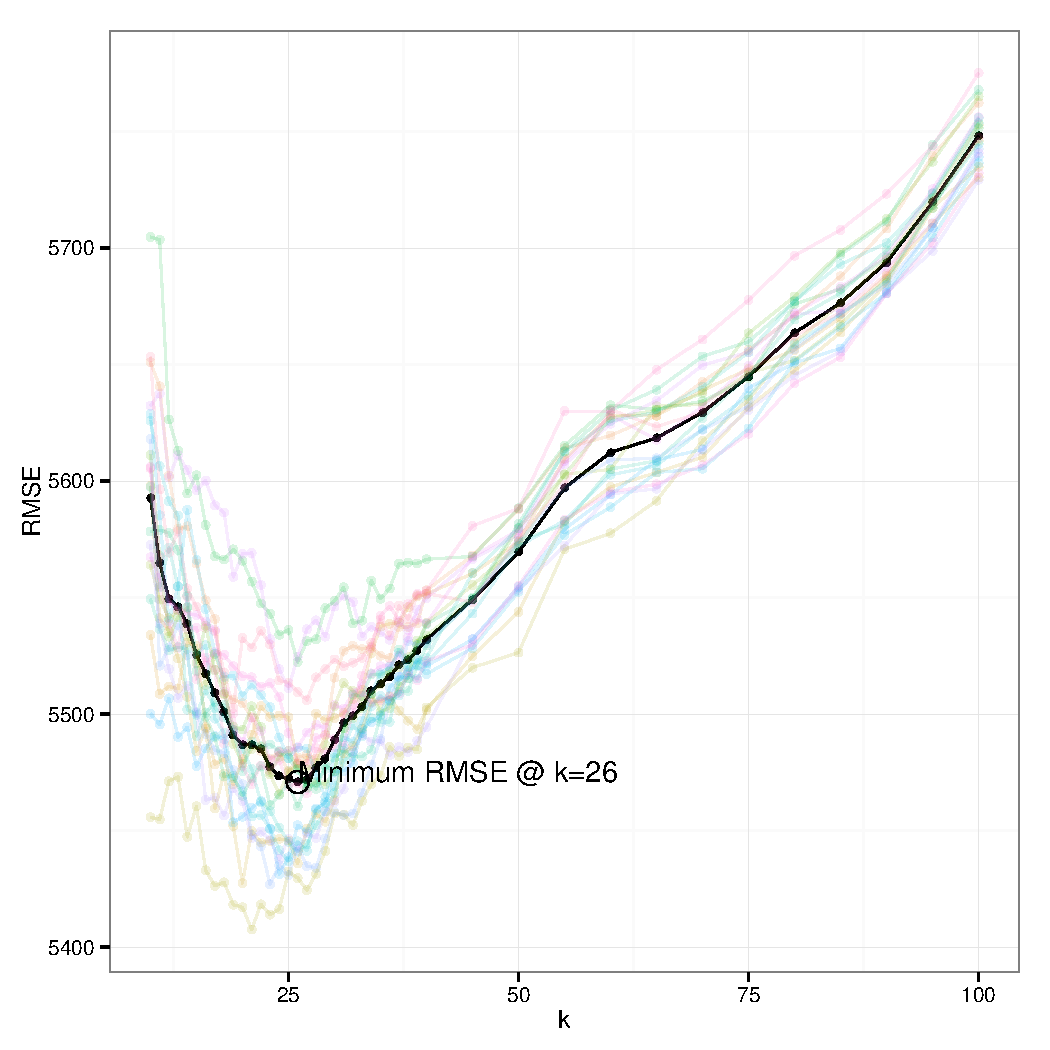
\includegraphics[scale=.5]{2p_cv_multi_k.pdf}
  \label{fig:2p_k_multi}
\end{figure}


\subsection{Price Predictions}
% latex table generated in R 3.2.2 by xtable 1.7-4 package
% Wed Oct  7 12:13:34 2015
\begin{table}[ht]
\centering
\begin{tabular}{rrrr}
  \hline
 & Year & Mileage & $\widehat{price}$ \\ 
  \hline
1 & 2008 & 75000 & 31678.22 \\ 
   \hline
\end{tabular}
\caption{Predicted Price with 2 Attributes} 
\label{tab:2p_predict}
\end{table}


\section{RMSE Comparison of kNN for 1 \& 2 Attributes}
\begin{figure}[!htb]
  \centering
  \caption{RMSE for 1 \& 2 Attributes}
  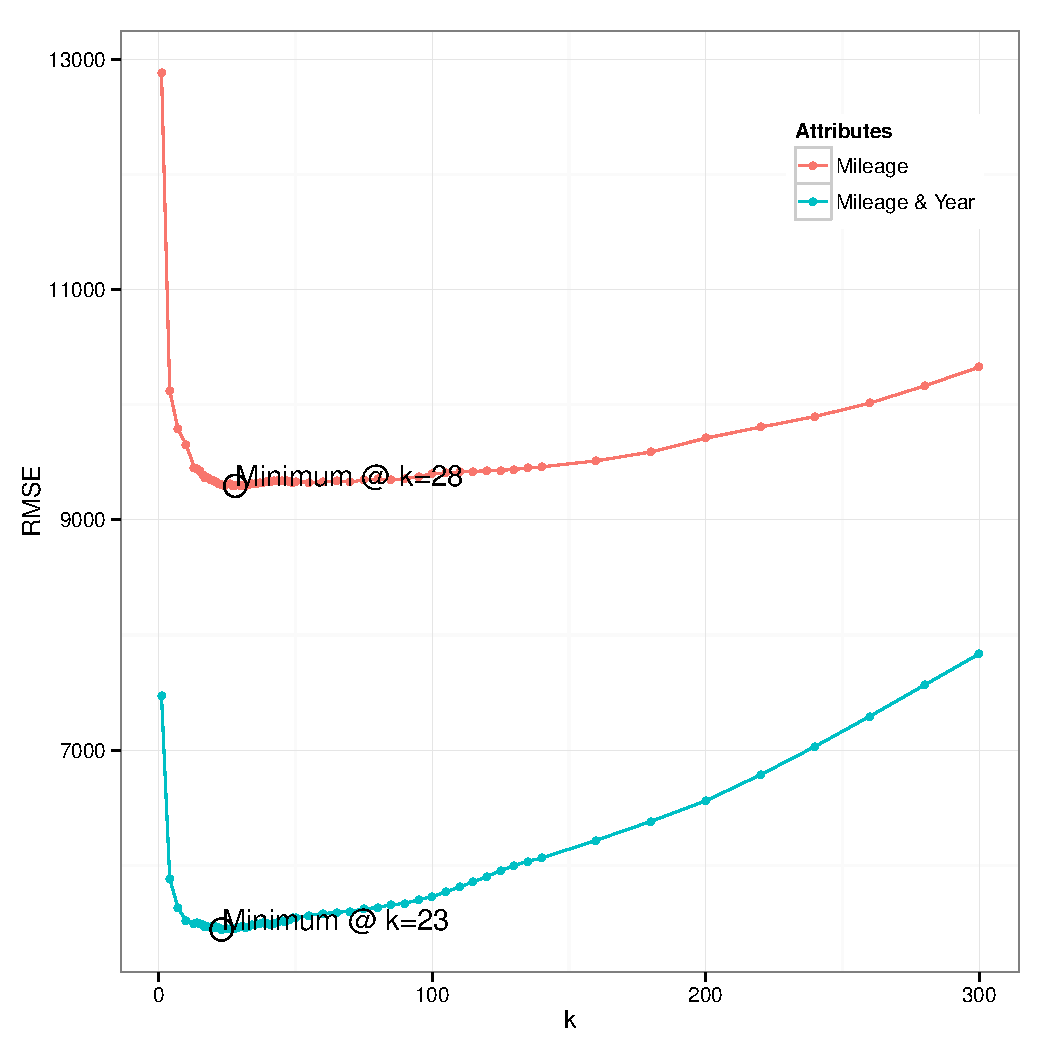
\includegraphics[scale=.5]{1p_2p_cv_compare.pdf}
  \label{fig:p_compare}
\end{figure}

\end{document}

% \input{.tex}

% \begin{figure}
%   \centering
%   \begin{subfigure}[b]{0.49\textwidth}
%     \caption{}
%     \includegraphics[width=\textwidth]{.pdf}
%     \label{fig:}
%   \end{subfigure}
%   \hfill
%   \begin{subfigure}[b]{0.49\textwidth}
%     \caption{}
%     \includegraphics[width=\textwidth]{.pdf}
%     \label{fig:}
%   \end{subfigure}
%   \caption{}
% \end{figure}

% \begin{figure}[!htb]
%   \centering
%   \caption{}
%   \includegraphics[scale=.5]{.pdf}
%   \label{fig:}
% \end{figure}

